\documentclass[a4apper,11pt]{article}

\usepackage{graphicx}
\usepackage{listings}
\usepackage{color}
\usepackage{hyperref}
\usepackage[table,xcdraw]{xcolor}
\usepackage{dirtree}

\hypersetup{
    colorlinks=true,
    linkcolor=black,
    filecolor=magenta,      
    urlcolor=blue,
}

\lstset{language=Prolog}

\definecolor{mygreen}{rgb}{0,0.6,0}
\definecolor{mygray}{rgb}{0.5,0.5,0.5}
\definecolor{mymauve}{rgb}{0.58,0,0.82}

\lstset{ 
  backgroundcolor=\color{white},   % choose the background color; you must add \usepackage{color} or \usepackage{xcolor}; should come as last argument
  basicstyle=\footnotesize,        % the size of the fonts that are used for the code
  breakatwhitespace=false,         % sets if automatic breaks should only happen at whitespace
  breaklines=true,                 % sets automatic line breaking
  captionpos=b,                    % sets the caption-position to bottom
  commentstyle=\color{mygreen},    % comment style
  deletekeywords={...},            % if you want to delete keywords from the given language
  escapeinside={\%*}{*)},          % if you want to add LaTeX within your code
  extendedchars=true,              % lets you use non-ASCII characters; for 8-bits encodings only, does not work with UTF-8
  firstnumber=0,                % start line enumeration with line 1000
  frame=none,	                   % adds a frame around the code
  keepspaces=true,                 % keeps spaces in text, useful for keeping indentation of code (possibly needs columns=flexible)
  keywordstyle=\color{blue},       % keyword style
  language=Prolog,                 % the language of the code
  morekeywords={*,...},            % if you want to add more keywords to the set
  numbers=right,                    % where to put the line-numbers; possible values are (none, left, right)
  numbersep=5pt,                   % how far the line-numbers are from the code
  numberstyle=\tiny\color{mygray}, % the style that is used for the line-numbers
  rulecolor=\color{black},         % if not set, the frame-color may be changed on line-breaks within not-black text (e.g. comments (green here))
  showspaces=false,                % show spaces everywhere adding particular underscores; it overrides 'showstringspaces'
  showstringspaces=false,          % underline spaces within strings only
  showtabs=false,                  % show tabs within strings adding particular underscores
  stepnumber=2,                    % the step between two line-numbers. If it's 1, each line will be numbered
  stringstyle=\color{mymauve},     % string literal style
  tabsize=2,	                   % sets default tabsize to 2 spaces
  title=\lstname                   % show the filename of files included with \lstinputlisting; also try caption instead of title
}

\title{Introduction to Artifficial Intelligence.\\ Assignment I: Humans vs Orcs Rugby.}
\author{Murashko Alecsey,\\ Group 6}

\begin{document}
\maketitle
\newpage
\tableofcontents

\newpage
\section{Assignment Assumptions and Testing}
\subsection{Assignment Assumptions}
During the implementation of the Assignment, I have made few assumptions according to the assignment description.
\begin{enumerate}
    \item The field is $20 \times 20$ squares.
    \item The player currently holding the ball is called Runner.
    \item Runner can move one square up, down, left or right.
    \item Runner can not go beyond the field's boundaries.
    \item If Runner tries to step in the square occupied by another player, then the step will not be counted, whereas will be printed out. Moreover, the step performance mechanism is depicted in Figure \ref{pic:stepInPlayer}.
    \item The random search takes 100 steps to perform, and if it does not find the solution - it terminates.
    \item The Implementation may not be 100\% correct and complete, but the places where implementation is not complete are emphasized in the text.
    \item The algorithm's Implementation may cause side effects in the instance of the program running. Thus, it is recommended to restart the program after one attempt to solve the problem was performed.
    \item Code Examples provided here differ from the actual code itself for clearness and shortness.
\end{enumerate}

\begin{figure}[h]
    \centering
    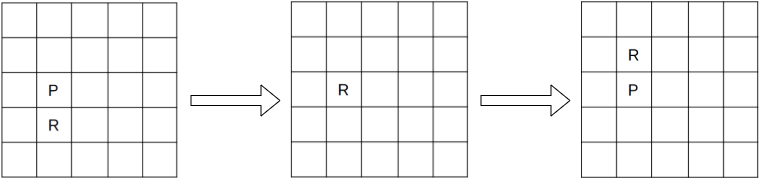
\includegraphics[width=0.9\textwidth]{pic/MoveInSquareWithPlayer.png}
    \caption{Positions of players by performing $move(1,2) \rightarrow move(1,3)$.}
    \label{pic:stepInPlayer}
\end{figure}

\subsection{Testing}
The Report itself shows the results of how algorithms perform on the map depicted in Figure \ref{pic:TCMap}. Statistical analysis was performed on the test cases provided with the report in the folder $Test\_Input$.

\begin{figure}[h]
    \centering
    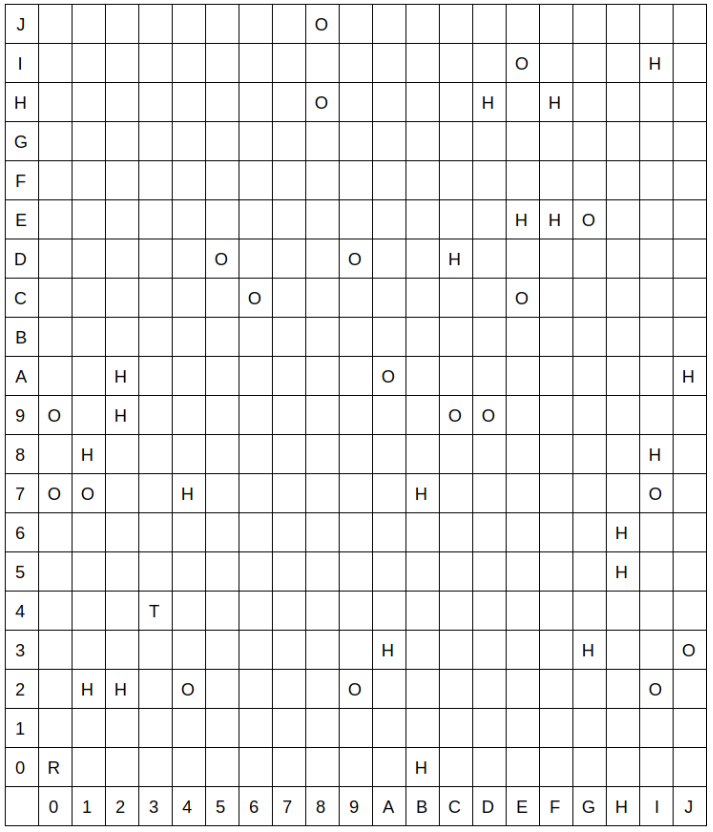
\includegraphics[width=0.9\textwidth]{pic/TestMap.png}
    \caption{Test Cases Map}
    \label{pic:TCMap}
\end{figure}

The output of the programs is done as array of objects in the form $p(x,y)$ or $m(x,y)$,  where $p(x,y)$ stands for ``The ball was passed(thrown) to position x,y'' and $m(x,y)$ stands for ``Runner moved to position x,y''.

\newpage
\section{Random Search}
\subsection{Basic Idea}

The Random Search Algorithm is implemented in recursive manner. All the predicates are recursively calling each other with different arguments. For instance, \[solve\_game\_random(Pos\_x, Pos\_y, Steps, Nsteps, Max\_steps)\]is the main function -- function where the recursion begins. It may call other functions, such as \[throw\_up\_right(Pos\_x, Pos\_y, Steps, Nsteps, Max\_steps)\] or \[move\_up(Pos\_x, Pos\_y, Steps, Nsteps, Max\_steps)\] which will determine, whether the Action can be performed, and if so -- will change the variables $Pos\_x, Pos\_y, Steps, Nsteps, Max\_steps$ accordingly, and call \[solve\_game\_random(Pos\_x, Pos\_y, Steps, Nsteps, Max\_steps)\] with new values of variables $Pos\_x, Pos\_y, Steps, Nsteps, Max\_steps$.
The variables, taken by all the functions play different roles:
\begin{itemize}
    \item $Pos\_x$ and $Pos\_y$ describe current position.
    \item $Steps$ is the array of already performed steps.
    \item $Nsteps$ is the number of performed steps.
    \item $Max\_steps$ is the amount of steps that can be made in current state.
\end{itemize}

\subsection{Code Examples}
Let us take a look at examples of the code. Listing \ref{random:base} shows how recursion base cases are implemented.

\begin{lstlisting}[caption={Recursion Base Cases.}, label={random:base}]
    solve_game_random(_,_,_,_,0):-
        format('Was not able to solve!).
    
    solve_game_random(Pos_x, Pos_y, Steps, Nsteps, Max_steps) :- 
    (
        t(Pos_x, Pos_y),
        format('ANSWER:~w~nNumSteps: ~w~n',[Steps,Nsteps])
    ).
\end{lstlisting}

The main idea of the algorithm is to compute two random numbers - $Action$ and $Direction$. If $Action = 1$, then move is performed -- $Direction \in [0,3]$, if $Action = 2$, ball throw is performed and $Direction \in [0,7]$. The part of the code responsible for it is shown in Listing \ref{random:moveSel}.

\begin{lstlisting}[caption={Recursion Move Selection.}, label={random:moveSel}]
random_between(1,2, Action), 
Action is 1,
random(0,4,Direction),
(
    Direction is 0 -> 
        move_up(Pos_x, Pos_y, Steps, Nsteps, Max_steps);
    Direction is 1 -> 
        move_right(Pos_x, Pos_y, Steps, Nsteps, Max_steps);
    % ----------------------- // -------------------------
    solve_game_random(Pos_x, Pos_y, Steps, Nsteps, Max_steps)
)
\end{lstlisting}

\subsection{Testing}
The Algorithm was tested on different test cases, but for now I will show the result of testing on map depicted in Figure \ref{pic:TCMap}.
After trying to run the algorithm several times, seeing messages of the form:
\begin{lstlisting}
Was not able to solve!
% 4,273 inferences, 0.001 CPU in 0.001 seconds (99% CPU, 3644455 Lips)
\end{lstlisting}

\noindent I finally got the answer:
\begin{lstlisting}
###### ANSWER: ######
[m(1,0),m(0,0),p(11,0),m(11,1),m(10,1),m(10,0),m(9,0),m(8,0),
    m(7,0),m(6,0),m(5,0),m(4,0),m(3,0),m(3,1),m(3,2),
    m(3,3),m(3,4)]
With Number of Steps: 16
#####################

% 1,857 inferences, 0.003 CPU in 0.003 seconds (99% CPU, 663188 Lips)    
\end{lstlisting}

\subsection{2 Yards Vision}
As far as my algrorithm does not depend on how far my agent can see, new ability will not affect the performance of my agent. So, there is no map which will be unsolvable with this new abolity or which is solvable with it, whereas it was unsolvable without it.

\subsection{Hard and Impossible to Solve Maps}
As the algorithm performs random search it is possible for it to solve any solvable map. The only hard situation which can happen in reality is the situation in which the shortest path takes more than 100 steps, but this issue can be solved by performing the following change in code:

\begin{lstlisting}
    % From:
    solve() :- time(solve_game_random(0, 0, [], 0, 100)).

    % To:
    solve() :- time(solve_game_random(0, 0, [], 0, 400)).
\end{lstlisting}

\subsection{Known bugs and issues to solve}
The Random Search algorithm has two bugs.
\begin{itemize}
    \item It can sometimes perform throwing a ball through the player to another player. This issue can be solved by adding additional verification in all the $throw\_*$ functions(As it is in backtracking and greedy algorithms), but it requires to rewrite vast amount of existing code.
    \item Dirty program architecture, due to its Imperative, but not Declarative nature.
    \item The Program generates side effects, so you a required to restart a program whenever you are trying to find the solution, using $solve().$
\end{itemize}

\subsection{Conclusion}
The Random Search algorithm is the most unreliable search algorithm, which is easy to code(at least, in imperative programming way). Can be used in different applications as temporary solution for the pathfinding problem.

\newpage
\section{Backtracking}
\subsection{Basic Idea}

Basic Idea of Backtracking implementation is to create knowledge base with rules, which will be able to automatically find the solution, using prolog tree. An example of implementation of sudoku solver, using this approach can be found \href{https://www.youtube.com/watch?v=5KUdEZTu06o&list=PLEvH6T-1oh76ndUiFUDjIyrrL9FyrSKXw&index=4}{Here}.


\subsection{Code Examples}
The codebase for the Backtracking implementation consists of two files -- $General\_Base.pl$ and $backtracking.pl$. First file contains common knowledge base for backtracking and greedy search, as well as different libraries used. Second file contains rule $satisfy(Curr, Moves, Passed, Visited)$, which checks whether it is possible to go from $Curr$ to the Tauchdown, by following path in $Moves$. Variables $Passed$ and $Visited$ are used by backtracking's logic and for debug. The main predicate is shown in Listig \ref{backtracking:base}.

\begin{lstlisting}[caption={Main Backtracking Predicate.}, label={backtracking:base}]
satisfy(Curr, _, _, _) :-
    Curr = [X0,Y0],
    t(X0,Y0).

satisfy(Curr, Moves, Passed, Visited):- (
	% Obtain X_0, X_1, Y_0, Y_1 from Curr and Moves:
    Curr = [X0,Y0],
    Moves = [[X1,Y1]|R],

    % Check whether current position is available:
    not(o(X0,Y0)),

    length(Moves, X), X #< 50, % Len(Moves) < 50:
    
    % Check two cases: 
    % If |(X0 + Y0)| - |(X1 + Y1)| = 1 => move()
    % Otherwise => pass()
    (
        (
            1 #= abs(X1-X0) + abs(Y1-Y0),
            move(Curr, [X1,Y1]),
            append(Visited, [[X1,Y1]], Vis),
            satisfy([X1,Y1], R, Passed, Vis)
        ); (
            Passed #= 0,
            pass(Curr, [X1,Y1]),
            append(Visited, [[X1,Y1]], Vis),
            satisfy([X1,Y1], R, 1, Vis)
        )
    )
).    
\end{lstlisting}

As you can see from the code listing, this time main predicate is written fully declarative, as well as all the other predicates.

\subsection{Testing}
The backtracking algorithm finds the solution for the map depicted in Figure \ref{pic:TCMap}:
\begin{lstlisting}
% 1,952,491 inferences, 0.106 CPU in 0.106 seconds (100% CPU, 18366271 Lips)
Answer: [p(2,2),m(2,3),m(2,4),m(3,4)], with the number of Steps: 4
true. 
\end{lstlisting}

\subsection{2 Yards Vision}
As with the Random search algorithm my backtracking does not depend on the radius of vision of my agent. Thus, there is no map which will be unsolvable with this new abolity or which is solvable with it, whereas it was unsolvable without it.

\subsection{Hard and Impossible to solve maps}
The only limitation of the algorithm is the size of the map. The algorithm works well and finds the solution in reasonable amount of time only for small maps, or in cases when tauchdown is in somewhat favorable position\footnote{There is no need to perform big amount of steps to get to the tauchdown.}.

\subsection{Conclusion}
Backtracking algorithm always finds one of the optimal solutions, but requires very big amount of time and computational resources. Can be used to solve constraint satisfaction problems or search problems in small search space.

\newpage
\section{Greedy Algorithm}
\subsection{Basic Idea}

The basic idea of the Greedy Algorithm is to use a heuristic function to decide on each step where to go. I've used manhattan heuristic to create my heuristic function. The implementation of the greedy algorithm is imperative and uses recursion, so it looks pretty like the implementation on Python or any other imperative language.

\subsection{Code Examples}

\begin{lstlisting}[caption={Main Greedy Predicate.}, label={greedy:base}]
greedy(Curr, Moves, _,_):-
	Curr = [X,Y],
    t(X,Y),
    parse([0,0],Moves, 0, []), !.

greedy(Curr, Moves, Passed, Queue):-
	expand_nodes(Curr, Q1, Passed),
    append(Queue, Q1, Q2),
    minNode(Q2, MinNode, NewQueue),
    MinNode = [_, NextPos],
    (
        (
            (
                (
                    (
                        Curr = [Xc,Yc],
                        NextPos = [Xn, Yn],
                        1 #= abs(Xc-Xn) + abs(Yc - Yn),
                        NewPassed = Passed
                    );(
                        Passed #= 0,
                        pass(Curr, NextPos),
                        NewPassed #= 1
                    )
                )
            ),
            append(Moves, [NextPos], NewMoves),
            greedy(NextPos, NewMoves, NewPassed, NewQueue)
        ); (
            greedy(NextPos, Moves, Passed, NewQueue)
        )
    ).
\end{lstlisting}
    

My implementation uses queue, which is implemented as a list with one additional function: $minNode(Queue, MinNode, NewQueue)$, which takes $Queue$, find min node in it, deletes it from the $Queue$, and stores new queue and minimal node in $NewQueue$ and $MinNode$. 

Another important predicate here is $expand\_nodes(Curr, Queue, Passed)$, which looks for squares reachable from current position and adds them to the $Queue$ with corresponding heuristic values.

The main predicate of the program is shown in Listing \ref{greedy:base}. What it does is expands positions reachable from the current one, searches for the best one to take\footnote{With the minimum heuristic value.} and calls $greedy(...)$ with this minimal node.


\subsection{Testing}
The greedy algorithm finds the solution for the map depicted in Figure \ref{pic:TCMap}:
\begin{lstlisting}
Answer: [p(2,2),m(2,3),m(2,4),m(3,4)], with the number of Steps: 4
% 63,655 inferences, 0.010 CPU in 0.017 seconds (55% CPU, 6670889 Lips)
true .
\end{lstlisting}

\subsection{2 Yards Vision}
As with the Random search and backtracking algorithms, my greedy search does not depend on the radius of vision of my agent. Thus, there is no map which will be unsolvable with this new abolity or which is solvable with it, whereas it was unsolvable without it.

\subsection{Hard or impossible to solve maps}
For this algorithm, it is hard to solve maps where the agent is required to accomplish the move, which will have bigger cost than others. In this case, the algorithm will be able to solve the problem\footnote{Because the Queue was used in the process of selecting the node.}, but the output will contain some redundant information. Fortunately, such maps are practically rare, but an example of such a map is depicted in Figure \ref{pic:hard-greedy}.

\begin{figure}[h]
    \centering
    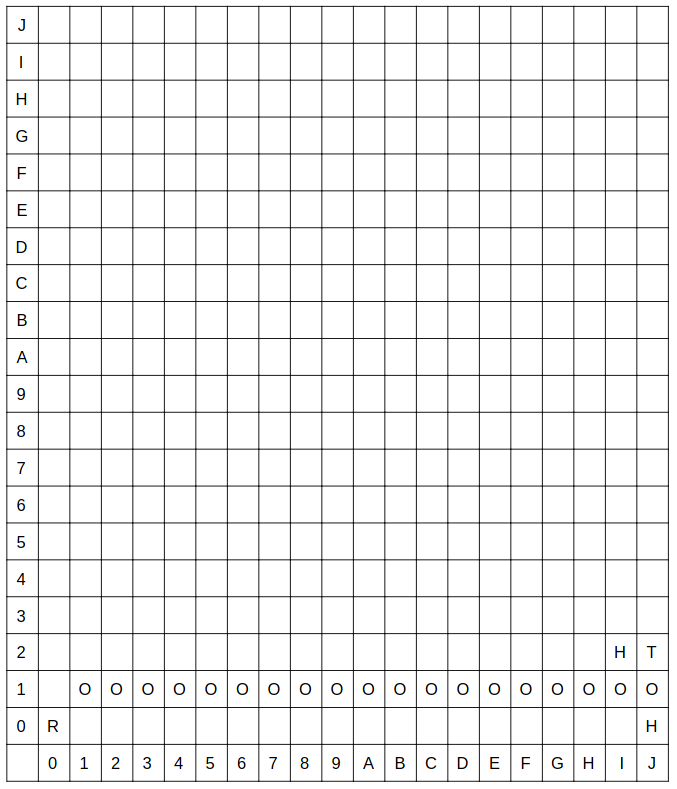
\includegraphics[width=0.7\textwidth]{pic/hard-greedy.png}
    \caption{Example of hard to solve map for Greedy Algorithm.}
    \label{pic:hard-greedy}
\end{figure}

\subsection{Conclusion}
Greedy algorithm is easy to implement, but it can not help you to surely find the shortest path. This algorithm, due to it's simplicity, can be used in practical applications, where you do not need to surely find the most optimal path(artifficial enemies in computer games).

\section{Simple Statistical Analysis of the Search Algorithms}

This section shows the results of performance of different algorithms runned on 30 different test cases.

\subsection{Corner Cases}
I've tested my algorithms on different corner cases and obtainde the results shown in Figure \ref{pic:stat:corner}.

\begin{figure}[h]
    \centering
    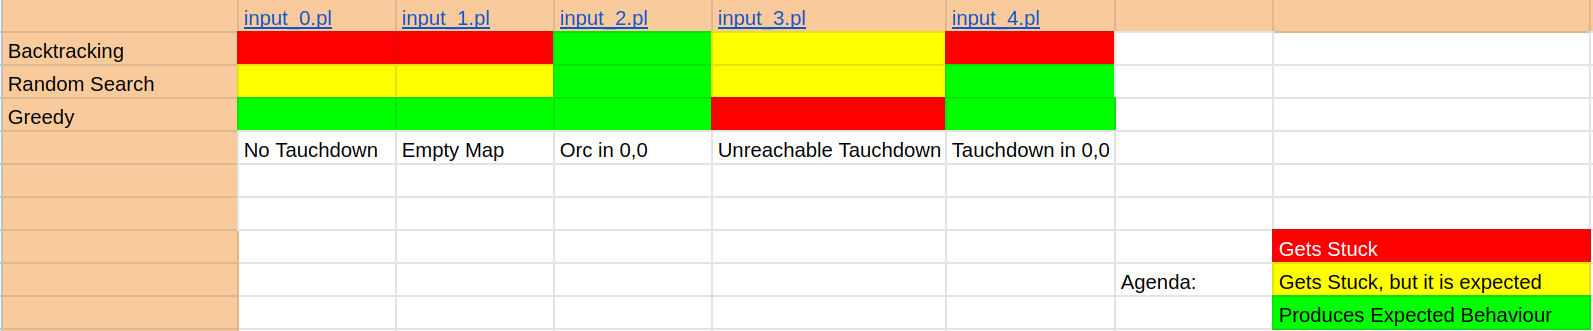
\includegraphics[width=0.9\textwidth]{pic/Corner_Cases.png}
    \caption{Corner Cases Statistics}
    \label{pic:stat:corner}
\end{figure}

As you can see from the Figure \ref{pic:stat:corner}, the most stable program is Greedy Search. Backtracking gets stuck, because it starts to encounter all the possible paths and this takes vast amount of time.

\subsection{Dense and Sparse Maps}
The following table shows the results of testing different algorithms on maps with big amount of objects. More complete information can be found \href{https://docs.google.com/spreadsheets/d/11Lfx49SPcEGMPLgSRwufFaIkQ5py8Cflug3j2oR3fC8/edit?usp=sharing}{here}.

\begin{table}[h]
    \begin{tabular}{lllll}
                        & input\_0.pl              & input\_1.pl              & input\_2.pl & input\_3.pl \\
    Backtracting Time   & 14.545                   & \cellcolor[HTML]{9B9B9B} & 0.350       & 6.368       \\
    Backtracting Length & 8                        & \cellcolor[HTML]{9B9B9B} & 4           & 7           \\
    Random Time         & \cellcolor[HTML]{9B9B9B} & 0.001                    & 0.001       & 0.001       \\
    Random Length       & \cellcolor[HTML]{9B9B9B} & 17                       & 18          & 23          \\
    Greedy Time         & 0.027                    & 0.07                     & 0.022       & 0.24        \\
    Greedy Length       & 10                       & 9                        & 4           & 11         
    \end{tabular}
\end{table}

Google sheets also contain results of tests on maps with 4 touchdowns and on maps with small amount of objects.

\subsection{Conclusion}
As you can see from this \href{https://docs.google.com/spreadsheets/d/11Lfx49SPcEGMPLgSRwufFaIkQ5py8Cflug3j2oR3fC8/edit?usp=sharing}{google sheet}, backtracking is not capabale of solving any probkem, because it takes him big amount of time, to accomplish the task. Greedy always finds the solution, but this solution is not always optimal, and random search algorithms finds the solution, if you are lucky enough.

\newpage
\appendix
\section{How to Run All the Algorithms}

When you unpack your archive, you will see the following structure:

\dirtree{%
.1 root.
.2 Automated map creation.
.3 src.
.4 Main.java.
.4 MapCreator.java.
.2 Implementation.
.3 Backtracking.
.4 backtracking.pl.
.3 Greedy Search.
.4 Greedy Search.pl.
.3 Random\_Search.
.4 random\_search.pl.
.3 Test\_Input.
}

$backtracking.pl$, $Greedy Search.pl$ and $random\_search.pl$ - should be executed in the following form:
\begin{lstlisting}
    swipl [Algorithm] [Input]
\end{lstlisting}

Example:
\begin{lstlisting}
    swipl swipl Greedy\ Search.pl ../Test_Input/Dense_1Td/input_2.pl 
\end{lstlisting}

When you are in SWI-Prolog Terminal, to get the solution, just type:

\begin{lstlisting}
    ?- solve().
\end{lstlisting}

\end{document}
